\documentclass[11pt]{article}

\usepackage[a4paper,margin=1in]{geometry}
\usepackage{amsmath}
\usepackage{amssymb}
\usepackage{amsfonts}
\usepackage{graphicx}
\usepackage{booktabs}
\usepackage{bm}
\usepackage[hidelinks]{hyperref}

% --- notation helpers ---
\newcommand{\E}{\mathbb{E}}
\newcommand{\Prob}{\mathbb{P}}
\newcommand{\eps}{\varepsilon}
\newcommand{\dd}{\,d}
\DeclareMathOperator{\Tr}{Tr}
\DeclareMathOperator*{\supop}{sup}

\title{Pairs Trading and Statistical Arbitrage Strategies}
\author{}
\date{}

\begin{document}
\maketitle

\noindent\textbf{Note.} This document is a faithful LaTeX reproduction of a chapter on pairs trading
and statistical arbitrage. The original PDF was compiled without its figures (every figure rendered as
an empty box). The eight figures here have been \emph{regenerated from code} in the accompanying
repository (\texttt{make\_book\_figures.py}, using the optimal-stopping solver \texttt{book\_opt.py}
and the backtest's own models); the optimal entry/exit trigger levels of Figure~\ref{fig:11_6} were
cross-validated against the trigger table printed later in the chapter.

\section{Pairs Trading and Statistical Arbitrage Strategies}

\subsection{Introduction}

The success of many trading algorithms depends on the quality of the predictions of stock price
movements. Predictions of the price of a single stock are generally less accurate than predictions of
a portfolio of stocks. A classical strategy which makes the most of the predictability of the joint,
rather than the individual, behaviour of two assets is \textbf{pairs trading}, where a portfolio
consisting of a linear combination of two assets is traded. At the heart of the strategy is how the
two assets co-move. As an example, take two assets whose spread, that is the difference between their
prices, exhibits a marked pattern and deviations from it are temporary. Then, pairs trading algorithms
profit from betting on the empirical fact that spread deviations tend to return to their historical or
predictable level. Thus, pairs trading falls under the class of strategies sometimes labeled as
\textbf{statistical arbitrage} (or StatArb for short). These are not true arbitrages (which are
strategies that produce returns in excess of the risk-free rate with zero risk), but rather are
strategies which bet off of the typical behaviour of asset prices, and hence are not risk-free.

\begin{figure}[ht]
  \centering
  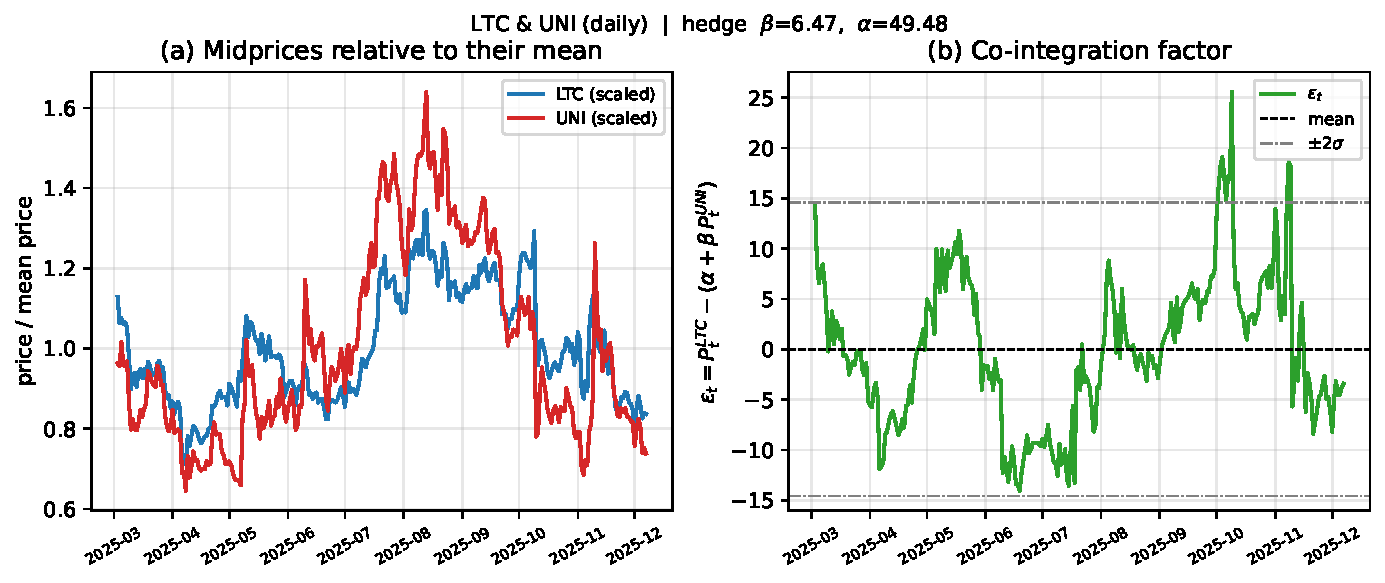
\includegraphics[width=\textwidth]{figures/fig_11_1.pdf}
  \caption{Two co-moving assets over a trading window: (left) midprices relative to their mean
  midprice; (right) the co-integration factor with its mean (dashed) and $\pm 2$ standard-deviation
  bands (dash-dotted). Here a real co-integrated crypto pair (LTC, UNI) stands in for the
  INTC/SMH example of the original text.}
  \label{fig:11_1}
\end{figure}

In Figure~\ref{fig:11_1} we show an example with two assets that tend to move together and in the same
direction. A portfolio consisting of long one asset and short the other will exhibit a less volatile
and more predictable behaviour than that of the individual assets. A more sophisticated approach is to
look at the co-integration factor of the prices of the two stocks: a path $\eps_t = A\,S^{(1)}_t +
B\,S^{(2)}_t$, where $A$ and $B$ are estimated from the data. If the mean-reverting behaviour is
persistent, we expect the value of a portfolio long $A$ shares of the first asset and short $|B|$
shares of the second to hover around the mean of the co-integration factor. A pairs trading strategy
then goes long the portfolio when it is `cheap' and closes the position when its value increases, or
goes short when it is `dear' and closes when its value decreases.

In Section~\ref{sec:adhoc} we show naive approaches which place ad hoc bands around the mean-reverting
level. In Section~\ref{sec:optimal} we develop approaches which determine the optimal bands to enter
and close a position, and in Section~\ref{sec:sta} the drifts of a collection of assets are
co-integrated.

\subsection{Ad Hoc Bands}\label{sec:adhoc}

A simple strategy to profit from the co-integration factor's mean-reversion is to place bands which
are one standard deviation above and below the mean-reverting level (here zero), and buy one unit of
the portfolio if the lower band is hit, or sell one unit if the upper band is hit. Once the strategy
has entered into a position, the next step is to close it: the strategy waits for the value of the
portfolio to be within a small interval, say $1/10$ of a standard deviation of the mean-reverting
level, and at that point liquidates.

\begin{figure}[ht]
  \centering
  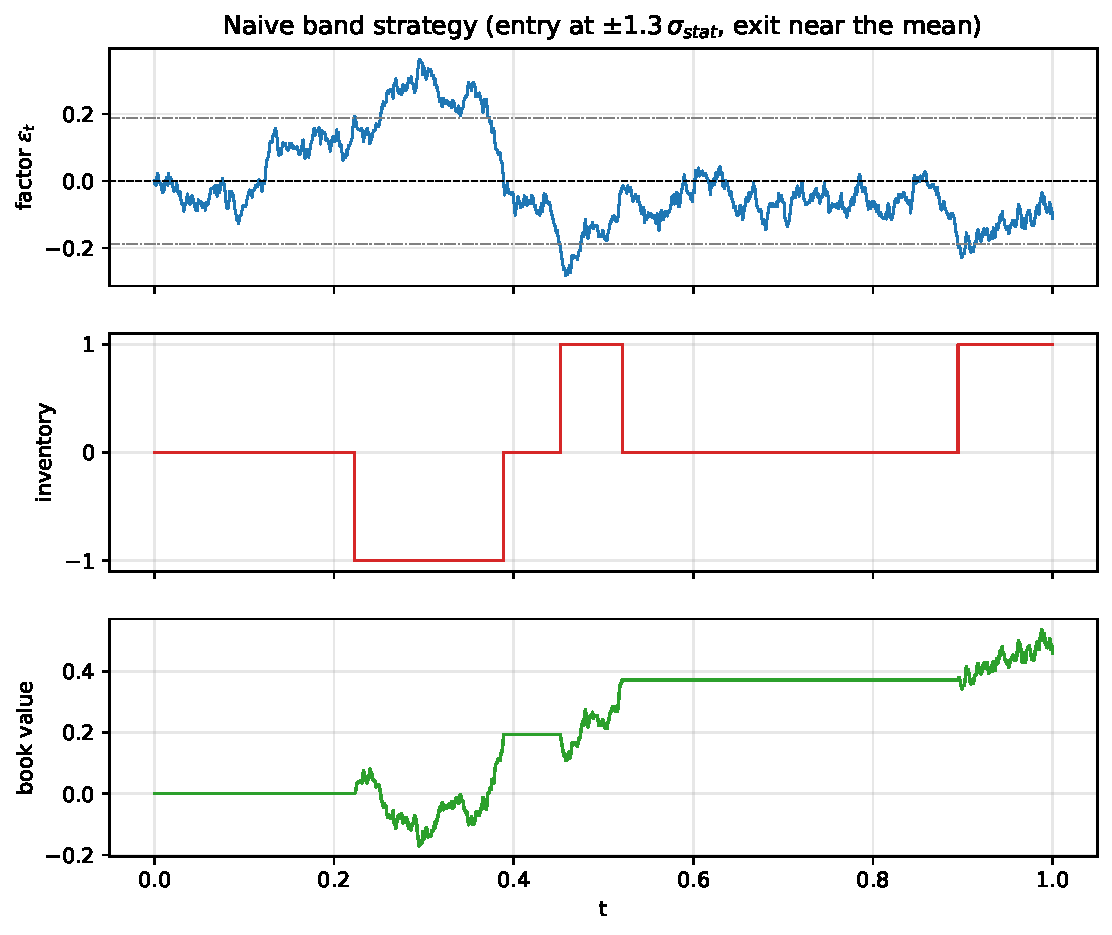
\includegraphics[width=0.8\textwidth]{figures/fig_11_2.pdf}
  \caption{A sample path of the co-integration factor, the trading position (inventory), and the
  book value of the trade, using a standard-deviation band strategy.}
  \label{fig:11_2}
\end{figure}

Figure~\ref{fig:11_2} shows three panels: a simulated sample path of the co-integration factor, the
inventory of the strategy as it opens and closes positions, and the accumulated book (marked-to-market)
value. The strategy waits for the path to breach an outer band, takes the corresponding position in
anticipation of mean-reversion, and holds the portfolio whose value fluctuates one-to-one with the
co-integration factor. The book value of the strategy is
\begin{equation}
  BV_t = X_t + \beta_t\left( A\,S^{(1)}_t + B\,S^{(2)}_t \right),
\end{equation}
where $X_t$ is the strategy's accumulated cash position and $\beta_t \in \{-1,0,1\}$ denotes the units
of the portfolio held. The strategy closes the position when the co-integration factor reverts to the
inner band, locking in a profit equal to the difference between the outer and inner bands.

In this scenario the agent ends with zero inventory, but this is not guaranteed: the strategy may have
entered a position which never reverts by the end of the trading horizon, inducing potential losses.
The wider the trigger bands, the more likely it is to end with inventory; wider bands have larger
profits when the position closes, but the co-integration factor makes fewer outer–inner band
transitions as the band size increases.

\begin{figure}[ht]
  \centering
  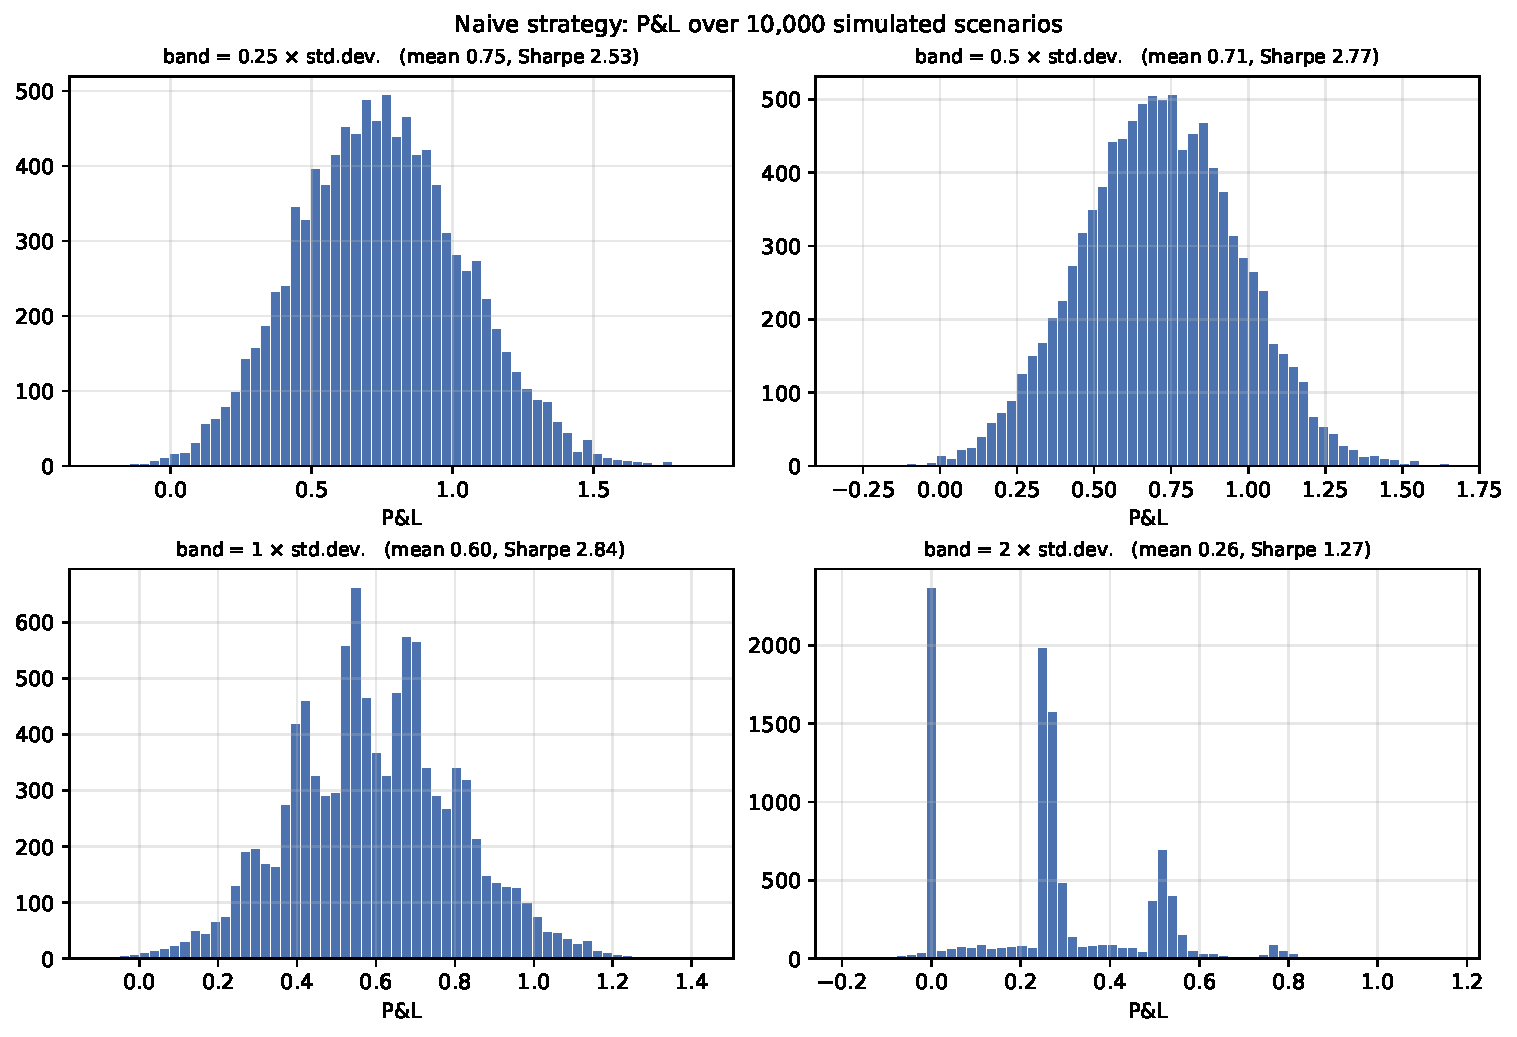
\includegraphics[width=\textwidth]{figures/fig_11_3.pdf}
  \caption{P\&L histograms from 10{,}000 simulated scenarios using the naive strategy with various
  trigger bands: (a) $0.25\times$, (b) $0.5\times$, (c) $1.0\times$, (d) $2.0\times$ the standard
  deviation. The Sharpe ratio first rises and then falls with the band size; the largest band yields
  a markedly multimodal distribution.}
  \label{fig:11_3}
\end{figure}

Figure~\ref{fig:11_3} shows the profit-and-loss (P\&L) histogram from generating 10{,}000 scenarios,
computing the co-integration factor and placing trades as described above. The Sharpe ratio (mean P\&L
divided by the standard deviation of P\&L) first increases as the band widens, but then starts
decreasing. Moreover, the distributions are multimodal: the profit from closing out a position equals
approximately the band size, so the P\&L concentrates near integer multiples of the band size, with the
weight on a given multiple equal to the probability of making that many round-trip trades during the
horizon. The P\&L is not concentrated solely on the band because, towards the end of the horizon, the
co-integration factor may not return to equilibrium, so the trader must close a position that makes less
profit than the band size, or may take a loss.

\subsection{Optimal Band Selection}\label{sec:optimal}

We now determine the optimal strategy to enter and exit by posing the problem as an optimal stopping
problem in which the trader makes a single round-trip trade and there is no terminal time horizon.
Assume the portfolio value (the co-integration factor) follows the Ornstein--Uhlenbeck dynamics
\begin{equation}
  d\eps_t = \kappa(\theta - \eps_t)\dd t + \sigma \dd W_t,
\end{equation}
with $W_t$ a standard Brownian motion. Here $\kappa$ is the rate of mean-reversion, $\theta$ the
long-run level, and $\sigma$ the volatility. The agent's performance criterion for exiting a long
position is
\begin{equation}
  H_+^{(\tau)}(t,\eps) = \E_{t,\eps}\!\left[ e^{-\rho(\tau - t)}(\eps_\tau - c) \right],
  \qquad
  H_+(t,\eps) = \supop_{\tau} H_+^{(\tau)}(t,\eps),
\end{equation}
where $c$ is the transaction cost for closing the portfolio and $\rho>0$ is the discount factor (an
urgency parameter: increasing $\rho$ pushes the exit boundary in towards the long-run level). The
performance criterion for entering a long position is
\begin{equation}
  G_+^{(\tau)}(t,\eps) = \E_{t,\eps}\!\left[ e^{-\rho(\tau - t)}\big(H_+(\tau,\eps_\tau) - \eps_\tau - c\big) \right],
  \qquad
  G_+(t,\eps) = \supop_{\tau} G_+^{(\tau)}(t,\eps);
\end{equation}
the agent pays $\eps + c$ for the portfolio but receives the exit option of value $H_+$.

Due to the stationarity of the OU process the value functions do not depend on time. The dynamic
programming principle implies that $H$ and $G$ satisfy the coupled variational inequalities
\begin{align}
  \max\big\{(\mathcal{L} - \rho)H_+(\eps)\,;\,(\eps - c) - H_+(\eps)\big\} &= 0,\\
  \max\big\{(\mathcal{L} - \rho)G_+(\eps)\,;\,(H_+(\eps) - \eps - c) - G_+(\eps)\big\} &= 0,
\end{align}
where $\mathcal{L}$ is the infinitesimal generator of the co-integration process,
\begin{equation}
  \mathcal{L} = \kappa(\theta - \eps)\,\partial_\eps + \tfrac{1}{2}\sigma^2\,\partial_{\eps\eps}.
\end{equation}

\subsubsection{The Optimal Exit Problem}

The variational inequality for $H$ resembles the value of a perpetual call option and is obtained by
finding the fundamental solutions of
\begin{equation}\label{eq:111}
  (\mathcal{L} - \rho)F(\eps) = 0, \tag{11.1}
\end{equation}
denoted $F_\pm(\eps)$, and writing $H_+(\eps) = A\,F_+(\eps) + B\,F_-(\eps)$ in the continuation region
($\eps < \eps^*$) and $H_+(\eps) = \eps - c$ in the exercise region ($\eps > \eps^*$). The value
matching and smooth pasting conditions are $H_+(\eps^*) = \eps^* - c$ and $\partial_\eps H_+(\eps^*)=1$.
The fundamental solutions are
\begin{equation}
  F_+(\eps) = \int_0^\infty u^{\frac{\rho}{\kappa}-1}\,
    e^{-\sqrt{\frac{2\kappa}{\sigma^2}}(\theta - \eps)u - \frac12 u^2}\dd u,
  \qquad
  F_-(\eps) = \int_0^\infty u^{\frac{\rho}{\kappa}-1}\,
    e^{+\sqrt{\frac{2\kappa}{\sigma^2}}(\theta - \eps)u - \frac12 u^2}\dd u.
\end{equation}
One can show that $F_+$ is strictly positive, increasing and convex, while $F_-$ is strictly positive,
decreasing and convex. The value function $H$ must vanish as $\eps \to -\infty$, hence $B=0$ and
\begin{equation}
  H_+(\eps) = A\,F_+(\eps)\,\mathbf{1}_{\eps<\eps^*} + (\eps - c)\,\mathbf{1}_{\eps\ge\eps^*}.
\end{equation}
Applying value matching and smooth pasting, $A\,F_+(\eps^*)=\eps^*-c$ and $A\,F_+'(\eps^*)=1$. Taking
the ratio, the optimal exit level is the unique solution of
\begin{equation}\label{eq:112}
  (\eps^* - c)\,F_+'(\eps^*) = F_+(\eps^*), \tag{11.2}
\end{equation}
and $A = (\eps^*-c)/F_+(\eps^*)$, so that
\begin{equation}
  H_+(\eps) = \frac{F_+(\eps)}{F_+(\eps^*)}(\eps^* - c)\,\mathbf{1}_{\eps<\eps^*}
    + (\eps - c)\,\mathbf{1}_{\eps\ge\eps^*}.
\end{equation}

\begin{figure}[ht]
  \centering
  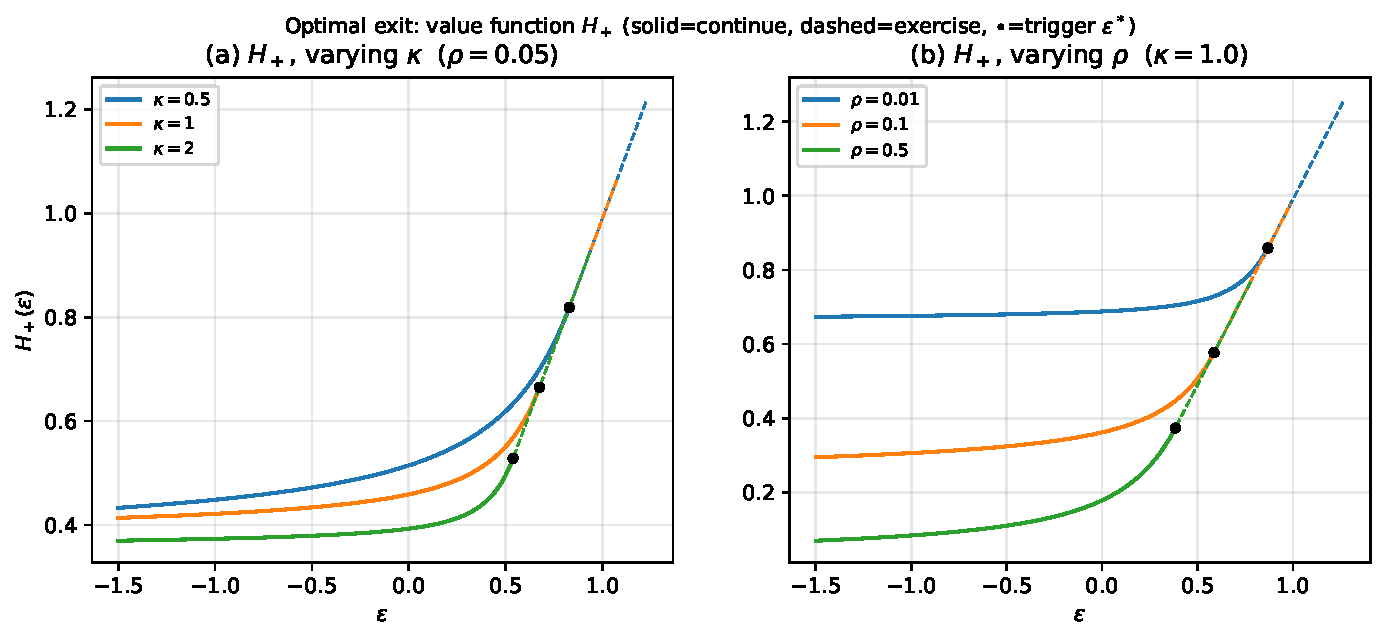
\includegraphics[width=\textwidth]{figures/fig_11_4.pdf}
  \caption{The optimal exit value function $H_+$ (solid in the continuation region, dashed in the
  exercise region) and the optimal exit triggers (circles), as the mean-reversion rate $\kappa$ and
  discount rate $\rho$ vary ($\theta=0$, $\sigma=0.5$, $c=0.01$).}
  \label{fig:11_4}
\end{figure}

Figure~\ref{fig:11_4} shows the value function as $\kappa$ and $\rho$ vary. As the mean-reversion rate
increases, the optimal trigger levels decrease, since the co-integration factor is drawn more strongly
to the mean-reversion level. Similarly, as $\rho$ increases, the trigger levels decrease, drawing the
stopping time nearer since future gains are discounted more.

\subsubsection{The Optimal Entry Problem}

Armed with the optimal exit strategy, we solve the entry problem, again a perpetual American-style
option but with exercise value $H_+(\eps) - \eps - c$. We anticipate $G_+$ decreasing in $\eps$ and
write
\begin{equation}
  G_+(\eps) = D\,F_-(\eps)\,\mathbf{1}_{\eps>\eps_*} + \big(H_+(\eps) - \eps - c\big)\,\mathbf{1}_{\eps\le\eps_*}.
\end{equation}
Value matching and smooth pasting give $D\,F_-(\eps_*) = H_+(\eps_*) - \eps_* - c$ and
$D\,F_-'(\eps_*) = H_+'(\eps_*) - 1$, hence the entry trigger solves
\begin{equation}\label{eq:113}
  \big(H_+(\eps_*) - \eps_* - c\big)F_-'(\eps_*) = \big(H_+'(\eps_*) - 1\big)F_-(\eps_*). \tag{11.3}
\end{equation}
Naturally $\eps_* < \eps^*$, and
\begin{equation}
  G_+(\eps) = \frac{F_-(\eps)}{F_-(\eps_*)}\big(H_+(\eps_*) - \eps_* - c\big)\mathbf{1}_{\eps>\eps_*}
    + \big(H_+(\eps) - \eps - c\big)\mathbf{1}_{\eps\le\eps_*}.
\end{equation}

\begin{figure}[ht]
  \centering
  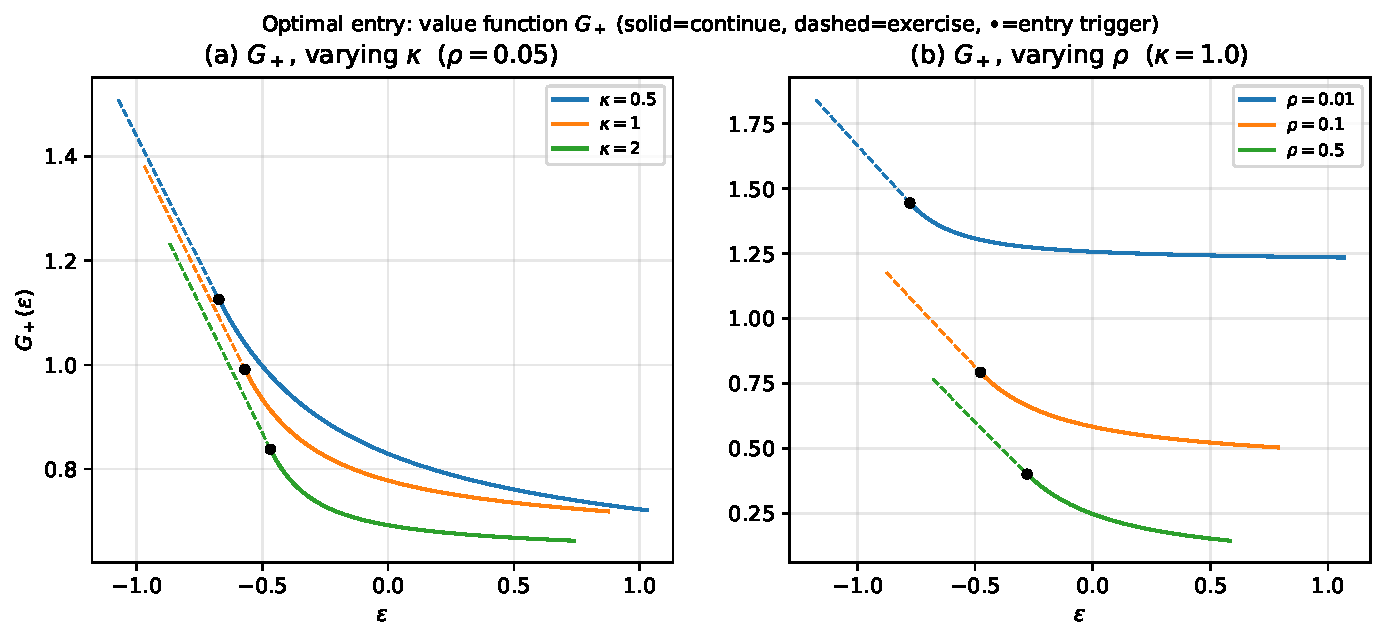
\includegraphics[width=\textwidth]{figures/fig_11_5.pdf}
  \caption{The optimal entry value function $G_+$ (solid in the continuation region, dashed in the
  exercise region) and the optimal entry triggers (circles), as $\kappa$ and $\rho$ vary
  ($\theta=0$, $\sigma=0.5$, $c=0.01$).}
  \label{fig:11_5}
\end{figure}

Figure~\ref{fig:11_5} shows $G_+$ as $\kappa$ and $\rho$ vary. As the mean-reversion rate increases,
the optimal entry triggers increase (move towards the mean-reversion level). Comparing
Figures~\ref{fig:11_5} and~\ref{fig:11_4}, the optimal entry and exit prices are not symmetric around
the mean-reversion level: the discount factor biases the entry point to occur closer to the
mean-reversion level relative to the exit point.

\subsubsection{Double-Sided Optimal Entry--Exit}

We now allow the agent to enter either a long or a short position and then optimally exit. The exit
performance criteria are
\begin{equation}
  H_+^{(\tau)}(t,\eps) = \E_{t,\eps}\big[e^{-\rho(\tau-t)}(\eps_\tau - c)\big],
  \qquad
  H_-^{(\tau)}(t,\eps) = \E_{t,\eps}\big[e^{-\rho(\tau-t)}(-\eps_\tau - c)\big],
\end{equation}
with value functions $H_\pm = \supop_\tau H_\pm^{(\tau)}$. Here $H_+$ coincides with the previous
section, so we focus on $H_-$, which is decreasing in $\eps$ and vanishes as $\eps \to \infty$:
\begin{equation}
  H_-(\eps) = A\,F_-(\eps)\,\mathbf{1}_{\eps>\eps^*_-} - (\eps + c)\,\mathbf{1}_{\eps\le\eps^*_-}.
\end{equation}
Value matching and smooth pasting yield $A\,F_-(\eps^*_-) = -(\eps^*_- + c)$ and
$A\,F_-'(\eps^*_-) = -1$, so the short exit trigger solves
\begin{equation}\label{eq:114}
  (\eps^*_- + c)\,F_-'(\eps^*_-) = F_-(\eps^*_-). \tag{11.4}
\end{equation}
In all, the exit value functions are
\begin{align}
  H_+(\eps) &= \frac{F_+(\eps)}{F_+(\eps^*_+)}(\eps^*_+ - c)\,\mathbf{1}_{\eps<\eps^*_+}
    + (\eps - c)\,\mathbf{1}_{\eps\ge\eps^*_+},\\
  H_-(\eps) &= -\frac{F_-(\eps)}{F_-(\eps^*_-)}(\eps^*_- + c)\,\mathbf{1}_{\eps>\eps^*_-}
    - (\eps + c)\,\mathbf{1}_{\eps\le\eps^*_-}.
\end{align}
In the continuation region of the entry problem $G$ is a linear combination of both fundamental
solutions, $G(\eps) = A\,F_+(\eps) + B\,F_-(\eps)$ between the two entry triggers, with $A,B$
determined by value matching and smooth pasting at both triggers. The optimal entry points are in fact
equal to the corresponding optimal exit point from the opposite portfolio: the entry point for the long
portfolio equals the exit point from the short position, and vice versa.

\begin{figure}[ht]
  \centering
  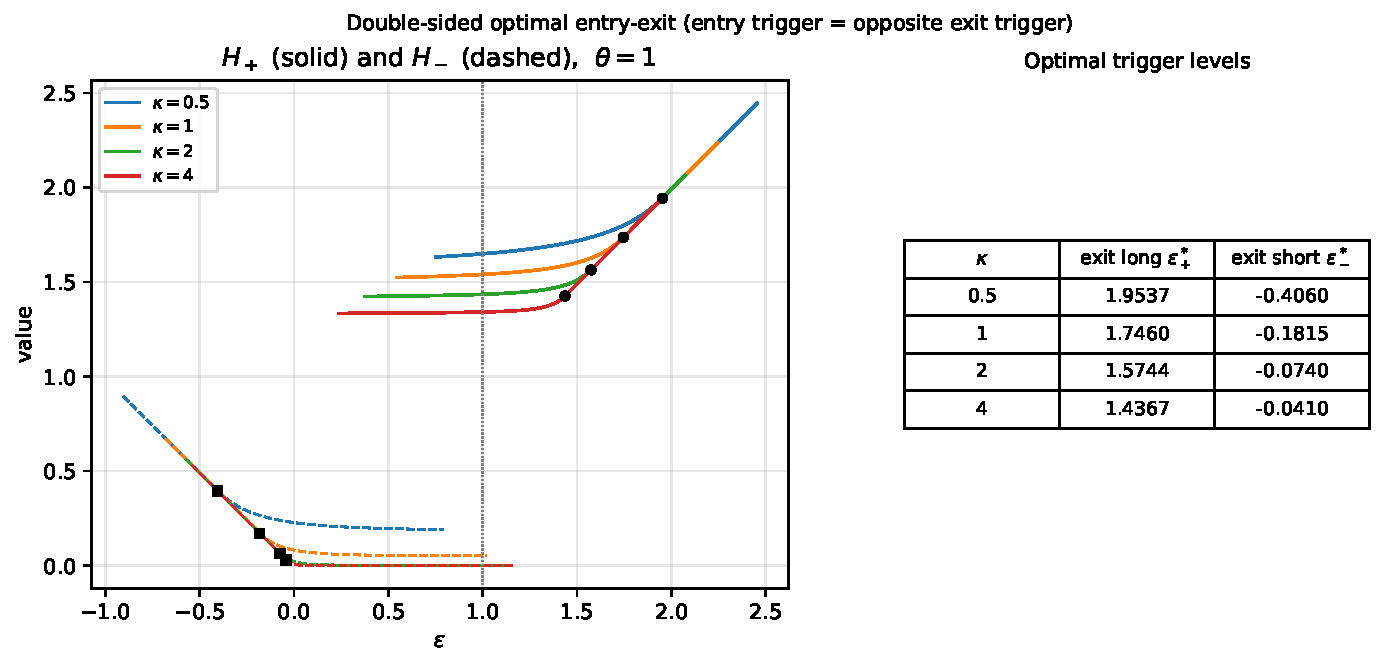
\includegraphics[width=\textwidth]{figures/fig_11_6.pdf}
  \caption{Double-sided problem: the value functions $H_+$ (solid) and $H_-$ (dashed) and the optimal
  trigger levels, as $\kappa$ varies ($\rho=0.01$, $\sigma=0.5$, $\theta=1$, $c=0.01$). Circles mark
  the long-exit triggers, squares the short-exit triggers; the table lists the computed values.}
  \label{fig:11_6}
\end{figure}

Figure~\ref{fig:11_6} shows the resulting value functions and triggers for $\rho=0.01$, $\sigma=0.5$,
$\theta=1$, $c=0.01$. The optimal exit points are not symmetric around $\theta$, and the optimal entry
points equal the corresponding optimal exit points from the opposite portfolio. The trigger levels are

\begin{table}[ht]
  \centering
  \begin{tabular}{ccccc}
    \toprule
    & \multicolumn{2}{c}{exit triggers} & \multicolumn{2}{c}{entry triggers}\\
    \cmidrule(lr){2-3}\cmidrule(lr){4-5}
    $\kappa$ & $\eps^*_+$ (long) & $\eps^*_-$ (short) & $\eps_{*+}$ (long) & $\eps_{*-}$ (short)\\
    \midrule
    0.5 & 1.9537 & $-0.4060$ & $-0.4060$ & 1.9537\\
    1.0 & 1.7460 & $-0.1815$ & $-0.1815$ & 1.7460\\
    2.0 & 1.5744 & $-0.0740$ & $-0.0740$ & 1.5744\\
    4.0 & 1.4367 & $-0.0410$ & $-0.0410$ & 1.4367\\
    \bottomrule
  \end{tabular}
  \caption{Optimal exit and entry triggers for the double-sided problem. These values are reproduced
  exactly by the repository's optimal-stopping solver (see \texttt{make\_book\_figures.py}).}
  \label{tab:triggers}
\end{table}

\section{Co-integrated Log Prices with Short-Term-Alpha}\label{sec:sta}

Another approach is one where the \emph{drifts} of a collection of assets are co-integrated, rather
than the prices themselves.

\subsection{Model Setup}

Suppose a collection of risky assets with price vector $Y = (Y^1_t,\dots,Y^n_t)_{0\le t\le T}$ satisfies
\begin{equation}\label{eq:115}
  \frac{dY^k_t}{Y^k_t} = \delta_k\,\alpha_t \dd t + \sum_{i=1}^n \sigma_{ki}\dd W^i_t,
  \qquad
  \alpha_t = a_0 + \sum_{i=1}^n a_i \log Y^i_t, \tag{11.5}
\end{equation}
with $W=(W^1,\dots,W^n)$ independent Brownian motions. The instantaneous covariance between assets $i$
and $j$ is $\Omega_{ij} = \sum_{k=1}^n \sigma_{ik}\sigma_{kj}$, so $\bm\sigma$ is the Cholesky factor of
$\bm\Omega = \bm\sigma\bm\sigma'$, assumed invertible. The quantity $\alpha_t$ acts as a co-integration
factor (a `short-term-alpha' component). Computing its differential,
\begin{equation}\label{eq:116}
  d\alpha_t = \kappa(\theta - \alpha_t)\dd t + \bm a'\bm\sigma \dd \bm W_t, \tag{11.6}
\end{equation}
with
\begin{equation}
  \kappa = -\sum_{k=1}^n a_k \delta_k = -\bm\delta'\bm a,
  \qquad
  \theta = \frac{\sum_{k=1}^n a_k \Omega_{kk}}{2\sum_{k=1}^n a_k\delta_k}
    = \frac{1}{2}\frac{\Tr(\bm A\bm\Omega)}{\bm\delta'\bm a},
\end{equation}
where $\bm A = \mathrm{diag}(\bm a)$. To ensure mean-reversion we assume $\bm\delta'\bm a < 0$. Writing
$\bm Z_t = \log \bm Y_t$, the log-prices form a (singular) vector-autoregressive model
$d\bm Z_t = (\bm c - \bm B\bm Z_t)\dd t + \bm\sigma\dd\bm W_t$.

We assume no price impact and optimise utility of terminal wealth. Let $\bm\pi =
(\pi^0_t,\dots,\pi^n_t)$ denote the dollar value invested in the riskless and risky assets; the number
of units held in asset $k$ is $m^k_t = \pi^k_t / Y^k_t$, and the wealth process is
$X^{\bm\pi}_t = \sum_{k=0}^n \pi^k_t = \sum_{k=0}^n m^k_t Y^k_t$, with
\begin{equation}
  dX^{\bm\pi}_t = (\bm\pi_t'\bm\delta)\,\alpha_t \dd t + \bm\pi_t'\bm\sigma \dd\bm W_t.
\end{equation}

\subsection{The Agent's Optimisation Problem}

The agent has exponential utility $u(x) = -e^{-\gamma x}$ and value function
\begin{equation*}
  H(t,x,\bm y) = \supop_{\bm\pi\in\mathcal A}\E_{t,x,\bm y}\big[-\exp(-\gamma X^{\bm\pi}_T)\big].
\end{equation*}
The dynamic programming equation is
\begin{equation}
  \partial_t H + \alpha\bm\delta'\bm D_{\bm y}H + \tfrac12 \bm D^{\bm\Omega}_{\bm{yy}}H
    + \supop_{\bm\pi}\Big\{(\bm\pi'\bm\delta)\alpha\,\partial_x H
    + \tfrac12(\bm\pi'\bm\Omega\bm\pi)\partial_{xx}H + \bm\pi'\bm\Omega\bm D_{\bm{xy}}H\Big\} = 0,
\end{equation}
subject to $H(T,x,\bm y) = -e^{-\gamma x}$. Completing the square gives the optimal investment in
feedback form,
\begin{equation}\label{eq:117}
  \bm\pi^* = -\frac{\bm\Omega^{-1}\bm\delta\,\alpha\,\partial_x H + \bm D_{\bm{xy}}H}{\partial_{xx}H}, \tag{11.7}
\end{equation}
and the non-linear PDE
\begin{equation}\label{eq:118}
  \partial_t H + \alpha\bm\delta'\bm D_{\bm y}H + \tfrac12 \bm D^{\bm\Omega}_{\bm{yy}}H
    - \frac{\mathcal{L}'H\,\bm\Omega^{-1}\mathcal{L}H}{2\,\partial_{xx}H} = 0. \tag{11.8}
\end{equation}

\subsection{Solving the DPE}

Motivated by the Merton problem, we posit
\begin{equation}
  H(t,x,\bm y) = -\exp\Big\{-\gamma\big(x + h(t,\alpha)\big) + \sum_{i=1}^n a_i \log y^i\Big\},
\end{equation}
with $\alpha = a_0 + \sum_i a_i \log y^i$ and $h(T,\alpha)=0$. Substituting and simplifying, the
non-linear terms cancel and $h$ satisfies a simple linear PDE,
\begin{equation}\label{eq:1110}
  \partial_t h - \tfrac12\Tr(\bm A\bm\Omega)\,\partial_\alpha h + \tfrac12(\bm a'\bm\Omega\bm a)\,
    \partial_{\alpha\alpha}h + \frac{\bm\delta'\bm\Omega\bm\delta}{2\gamma}\,\alpha^2 = 0, \tag{11.10}
\end{equation}
subject to $h(T,\alpha)=0$. The optimal investment becomes
\begin{equation}\label{eq:1111}
  \bm\pi^* = \frac1\gamma\big(\bm\Omega^{-1}\bm\delta\big)\alpha - \bm a\,\partial_\alpha h. \tag{11.11}
\end{equation}
The first term mirrors the classical Merton solution (with stochastic drift $\bm\delta\alpha_t$); the
second term, proportional to $\bm a$, is the correction due to co-integration.

\subsection{A Probabilistic Interpretation}

Under the risk-neutral measure $\Prob^*$ defined by the market price of risk
$\bm\lambda_t = -\bm\sigma^{-1}\bm\delta\,\alpha_t$, the co-integration factor becomes a
(driftless-in-level) Brownian motion,
\begin{equation}\label{eq:1113}
  d\alpha_t = -\tfrac12\Tr(\bm A\bm\Omega)\dd t + \bm a'\bm\sigma\dd\bm W^*_t. \tag{11.13}
\end{equation}
A Feynman--Kac argument then gives
\begin{equation}\label{eq:1114}
  h(t,\alpha) = \E^*_{t,\alpha}\!\left[\frac{\bm\delta'\bm\Omega\bm\delta}{2\gamma}\int_t^T \alpha_s^2\dd s\right], \tag{11.14}
\end{equation}
so the incremental value of trading the co-integrated collection is driven by the future expected
integrated $\alpha^2$, and increases with volatility (through $\bm\Omega$) and the strength
$\bm\delta$.

\subsection{Explicit Construction of the Optimal Investment Strategy}

Carrying out the expectation, $h(t,\alpha)$ is quadratic in $\alpha$, and the optimal investment takes
the explicit form
\begin{equation}\label{eq:1116}
  \bm\pi^* = \frac1\gamma\left\{(\bm\Omega^{-1}\bm\delta)\,\alpha
    + (\bm\delta'\bm\Omega\bm\delta)\Big[\tfrac12\tau\,\alpha + \tfrac14\Tr(\bm A\bm\Omega)\tau^2\Big]\bm a\right\},
  \qquad \tau = T-t. \tag{11.16}
\end{equation}
The first term is the Merton portfolio (the assets' drifts are $\bm\delta\alpha$); the second,
proportional to $\bm a$, is the co-integration correction, which decays as the terminal date
approaches --- the agent ignores the short-term-alpha effect as trading comes to a close.

\subsection{Numerical Experiments}

We showcase the strategy in a three-asset case with
\[
  \bm\delta = (1,1,0)', \quad \bm a = (-1,0,1)', \quad a_0 = 0,
\]
\[
  \bm\sigma = \begin{pmatrix} 0.2000 & 0 & 0\\ 0.0375 & 0.1452 & 0\\ 0.0250 & 0.0039 & 0.0967 \end{pmatrix}
  \;\Rightarrow\;
  \bm\Omega = \begin{pmatrix} 0.04 & 0.0075 & 0.005\\ 0.0075 & 0.0225 & 0.0015\\ 0.005 & 0.0015 & 0.01 \end{pmatrix},
\]
volatilities $\{2\%, 1.5\%, 1\%\}$, and initial prices $Y^1_0=11.10$, $Y^2_0=12.00$, $Y^3_0=11.00$. The
co-integration vector $\bm a$ implies only the first and third assets feed the factor, while $\bm\delta$
implies only the first and second assets' drifts are affected by it.

\begin{figure}[ht]
  \centering
  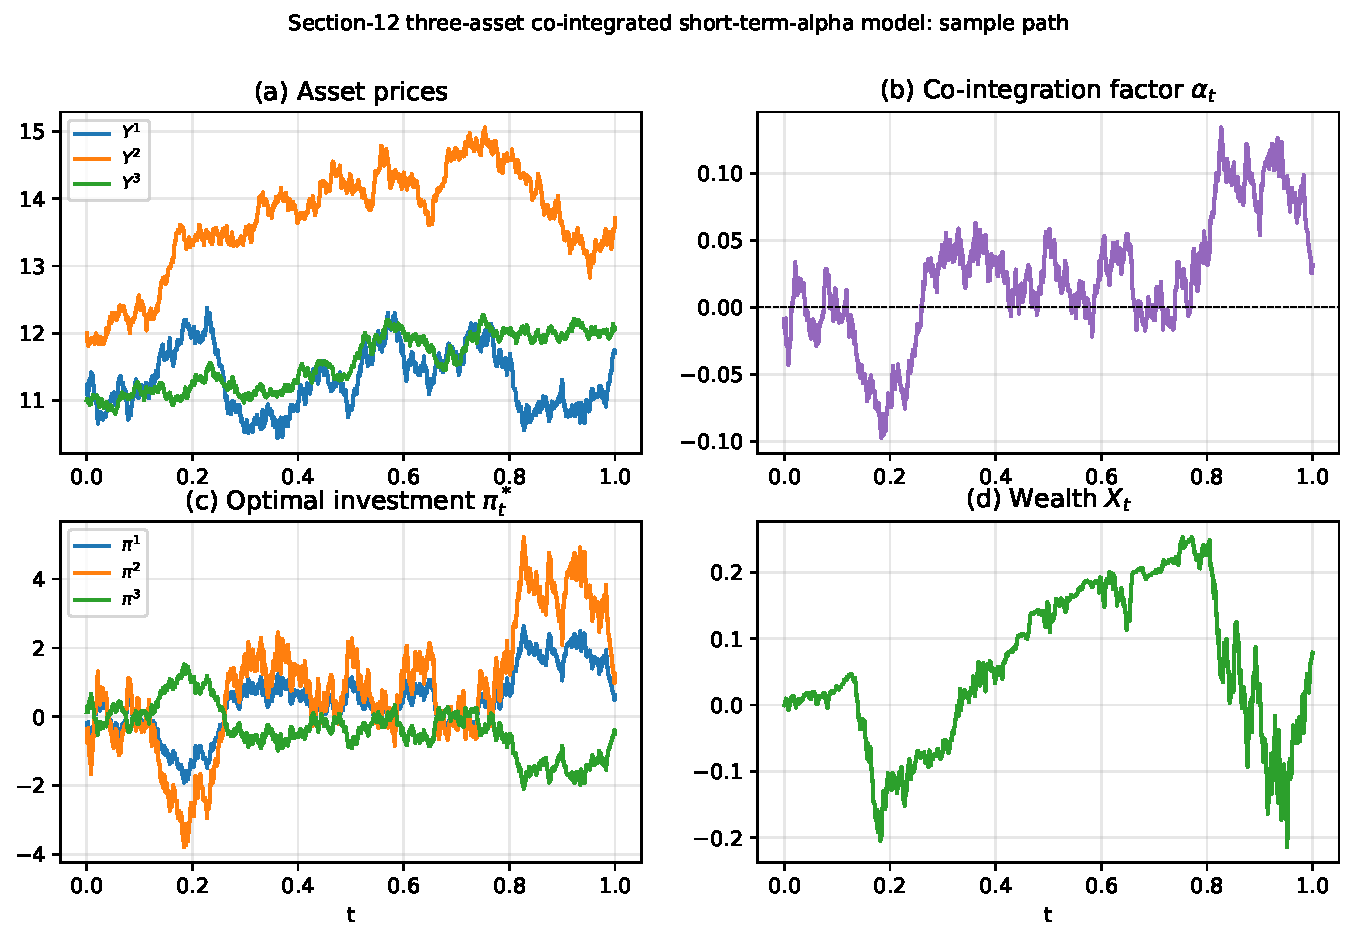
\includegraphics[width=\textwidth]{figures/fig_11_7.pdf}
  \caption{A single sample path of the co-integrated asset prices, the co-integration factor
  $\alpha_t$, the resulting optimal strategy $\bm\pi^*_t$, and the agent's wealth process $X_t$.}
  \label{fig:11_7}
\end{figure}

\begin{figure}[ht]
  \centering
  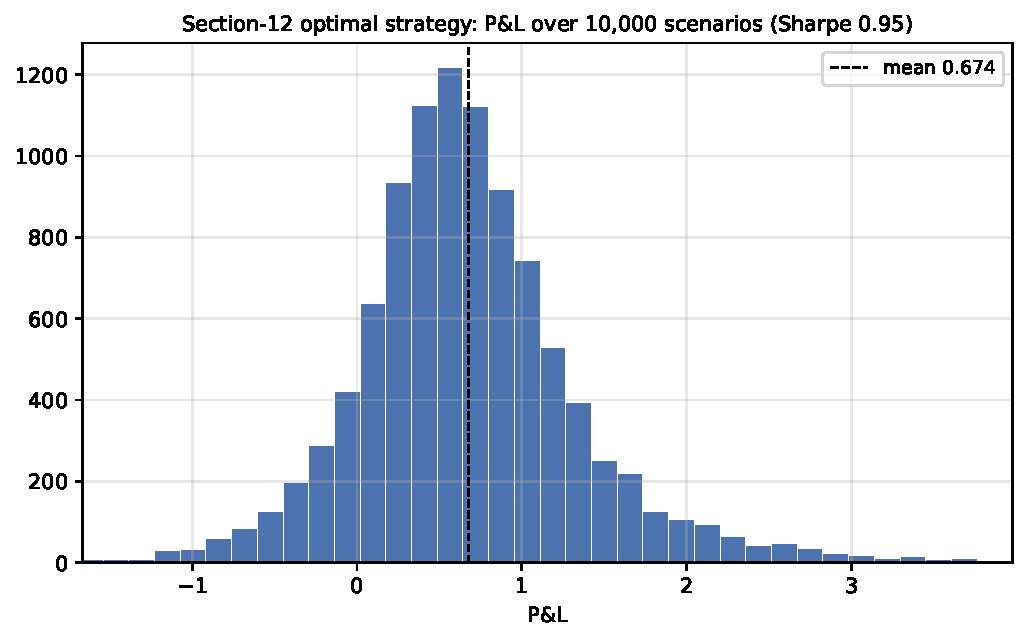
\includegraphics[width=0.75\textwidth]{figures/fig_11_8.pdf}
  \caption{Histogram of the P\&L of the optimal pairs trading strategy over many simulated scenarios.}
  \label{fig:11_8}
\end{figure}

Figure~\ref{fig:11_7} shows a sample path of the asset prices, co-integration factor, optimal strategy,
and wealth process. Figure~\ref{fig:11_8} shows the histogram of the terminal P\&L over many simulated
scenarios.

\section{Bibliography and Selected Readings}

Elliott, Van Der Hoek \& Malcolm (2005); Tourin \& Yan (2013); Leung \& Li (2014); Leung \& Ludkovski
(2011).

\end{document}
